\chapter{Supervised Learning} \label{chp:machinelearning}
\epigraph{People worry that computers will get too smart and take over the world, but the real problem is that they're too stupid and they've already taken over the world.}{Pedro Domingos, \cite{domingos_master_2015}}
\begin{figure}[H]
	\centering
	\copyrightbox[l]{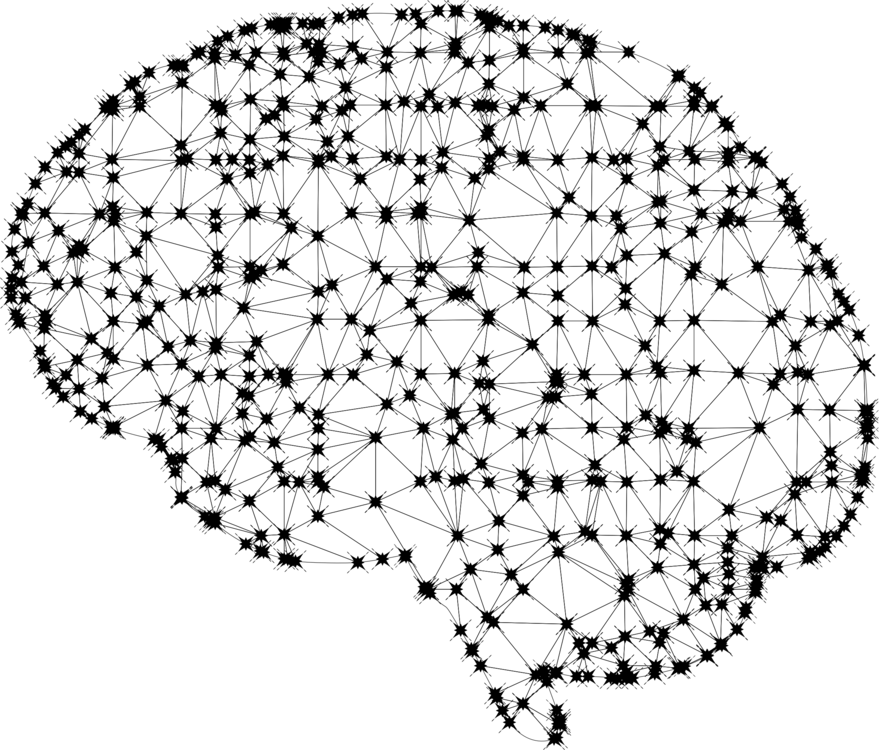
\includegraphics[scale=0.25]{../Images/brain.png}}{© Copyright trzcacak.rs}
	\caption{Artificial neural networks are inspired by neural networks in the brain. The figure is taken from \url{trzcacak.rs}.}
\end{figure}

% History
The use of the term \textit{machine learning} has exploded over the past years, and sometimes it even sounds like it is a new field. However, the truth is that many of the methods are relatively old, where for instance \textit{linear regression} was known in the early 19th century when \citet{legendre_nouvelles_1805} and \citet{gauss_theoria_1809} independently developed the concepts of mean square error (MSE). Those methods have just recently been taken under the machine learning umbrella, which is one of the reasons why the term is used more frequently than before. Another essential contributor to the booming popularity is the dramatic improvement of a majority of the machine learning algorithms, most notably neural networks, as discussed in the introduction.

% What is Machine Learning?
Unlike traditional algorithms, machine learning algorithms are not explicitly told what to do, but they use optimization tools to minimize a \textit{cost function} and fit a model to data sets. As a consequence, we often do not know precisely what the algorithms do and why they behave as they do. Because of this behavior and the fact that artificial neural networks are inspired by the human brain, the processing is often called artificial intelligence. As a definition of the term machine learning, we use the translation by Stanford University \cite{noauthor_machine_nodate}:

\begin{shadequote}{}
	Machine learning is the science of getting computers to act without being explicitly programmed.
\end{shadequote}

% Why Machine Learning?
In our search for a technique to solve quantum mechanical problems where less physical intuition is needed, machine learning appears as a natural tool. First, machine learning algorithms are able to provide impressive results, even with absence of rules specifying what the network should do. This was, for instance, demonstrated by \citet{silver2017mastering} who developed a chess engine which learned the rules by playing against itself thousands of times. Second, the fundamental goal of machine learning is to fit a model in order to minimize a cost function, which is exactly what we do in the popular variational Monte Carlo (VMC) method with the wave function as the model and with the energy as the cost function. However, in traditional VMC, the trial wave function is tailored to each particular system, which naturally requires a significant amount of physical intuition. With the trial wave function defined by a restricted Boltzmann machine (RBM), we attempt to find a model so flexible that it can approach the true wave function even with lack of physical intuition. This is important because the study of many urgent systems is out of reach for the existing methods due to lack of information about the wave function. Examples include bosonic systems, where expressions for the two-body correlations in general are unavailable \cite{holzmann_pair_1999}, and nuclear systems, where the three-body correlations are crucial \cite{sauer_three-nucleon_2014}.

% How do we use Machine Learning?
We typically classify the machine learning methods as either supervised or unsupervised, based on the way we define the cost function. Supervised models are provided with \textit{targets}, which are outputs that the model should obtain with a certain input data set. We then define the cost function as the error between the output from the model and the targets, and the model is trained until it is able to reproduce the targets. On the other hand, unsupervised models are not provided with targets, and the cost function thus needs to be defined in another way. In our work, we aim to construct a robust method for the study of the ground state of complex systems, and as targets for those systems usually are unavailable, we will use unsupervised algorithms. For RBMs, the cost function is traditionally defined by a system energy which we want to minimize. As there are many common concepts in supervised and unsupervised learning, we will in this chapter stick to supervised learning where we introduce essential concepts like artificial neurons, weights and optimization schemes. The Boltzmann machines, which are the models that we actually use in the work, are discussed in chapter \ref{chp:restricted}.

% The goal of supervised learning
Supervised learning maps an input to an output based on example input-output pairs. To make this work, we need to train the model such that the error between the targets and the outputs is tolerable small. However, this is in general not sufficient as we also want to make new predictions from the same model. The two points that need to be satisfied in supervised learning are therefore:
\begin{enumerate}
	\item The model needs to reproduce the targets
	\item The model should be able to fit future observations.
\end{enumerate}
In this chapter, we will examine how a model that satisfies both the requirements can be found, possible challenges and when the ansatz will break down. Subsequently, we will see that there is no guaranty that the second point is satisfied even when the first point is satisfied. First, the polynomial regression is presented to explain fundamental concepts of machine learning in an intuitive way, and thereafter we generalize the theory in form of linear regression. In the end, we go thorough neural networks which have many common features with the restricted Boltzmann machines discussed in the next chapter. 

\section{Polynomial regression}
The polynomial regression is perhaps the most intuitive example on supervised learning, as it can be used to solve problems everyone is familiar with. In general, polynomial regression finds the $p$'th degree polynomial, $f(x;\bs{c})=\sum_{i=0}^pc_ix^i$, that fits a set of points in the best possible way with $\bs{c}$ as the coefficients or \textit{estimators}. In two dimensions, the data set consists of some $n$ number of $x$- and $y$-coordinates,
\begin{align*}
\bs{x}&=(x_1,x_2,\hdots,x_n)\\
\bs{y}&=(y_1,y_2,\hdots,y_n),
\end{align*}
henceforth denoted by $\mathcal{D}=\{\bs{x},\bs{y}\}$. The data set can for instance be fitted to a second-order polynomial,
\begin{equation}
f(x;a,b,c)=ax^2+bx+c,
\end{equation}
where the parameters $a$, $b$ and $c$ are our estimators. The polynomial is now our model, and by evaluating it on all values in the $\bs{x}$-vector we obtain a set of $n$ equations
\begin{equation}
\mqty{
	\tilde{y}_1&=&ax_1^2&+&bx_1&+&c\\
	\tilde{y}_2&=&ax_2^2&+&bx_2&+&c\\
	\vdots&&\vdots&&\vdots&&\vdots\\
	\tilde{y}_n&=&ax_n^2&+&bx_n&+&c
}
\label{eq:lineareqs}
\end{equation}
where $\tilde{y}_i=f(x_i)$ is the output from the model with $x_i$ as the input. What we want to do is to determine the estimators $a$, $b$ and $c$ such that the mean squared error (MSE) of all these equations,
\begin{equation}
\min_{a,b,c}\frac{1}{n}\sum_{i=0}^{n-1}(y_i-f(x_i;a,b,c))^2,
\end{equation}
is minimized. The cost function, $\mathcal{C}(\bs{\theta})$, (also called the loss function) is then defined as the MSE, which is always the function that we try to minimize in machine learning. For our choice of model, the cost function reads
\begin{empheq}[box={\mybluebox[5pt]}]{equation}
\mathcal{C}(a,b,c)=\frac{1}{n}\sum_{i=0}^{n-1}\Big(y_i-(ax_i^2+bx_i+c)\Big)^2,
\end{empheq}
which can be minimized in several ways. Before we proceed to the minimization, we will introduce a more general notation, where the estimators are collected in a column vector 
\begin{equation}
\bs{\theta}\equiv(a,b,c)^T
\end{equation}
and the $x_i^j$'s are collected in a row vector
\begin{equation}
\bs{X}_i\equiv(x_i^2, x_i^1, x_i^0)=(x_i^2, x_i, 1).
\end{equation}
By using this, the cost function can be written as
\begin{equation}
\begin{aligned}
\mathcal{C}(\bs{\theta})&=\frac{1}{n}\sum_{i=0}^{n-1}\Big(y_i-\sum_{j=0}^2X_{ij}\theta_j\Big)^2\\
&=\frac{1}{n}\sum_{i=0}^{n-1}\Big(y_i-\bs{X}_i\bs{\theta}\Big)^2\\
&=\frac{1}{n}(\bs{y}-\bs{X}\bs{\theta})^T(\bs{y}-\bs{X}\bs{\theta})
\end{aligned}
\label{eq:polynomialcost}
\end{equation}
where we in the last step have collected all the vectors $\bs{X}_i$ in a matrix $\bs{X}=[\bs{X}_1,\bs{X}_2,\hdots,\bs{X}_n]$. As the minimum of the cost function with respect to an estimator $\theta_k$ is found when the derivative is zero, we need to solve the equation
\begin{equation}
\begin{aligned}
\frac{\partial \mathcal{C}(\bs{\theta})}{\partial\theta_k} &=\frac{\partial}{\partial\theta_k}\bigg(\frac{1}{n}\sum_{i=0}^{n-1}\Big(y_i-\sum_{j=0}^2X_{ij}\theta_j\Big)^2\bigg)\\
&=\frac{2}{n}\sum_{i=0}^{n-1}X_{ik}\Big(y_i-\sum_{j=0}^2X_{ij}\theta_j\Big)=0.
\end{aligned}
\end{equation}
We can go further and write it on matrix-vector form as
\begin{equation}
\frac{\partial \mathcal{C}(\bs{\theta})}{\partial\bs{\theta}}=\frac{2}{n}\bs{X}^T(\bs{y}-\bs{X}\bs{\theta})=0
\end{equation}
where the differentiating is done element-wise, $\partial\mathcal{C(\bs{\theta})}/\partial\theta_k$. This is satisfied if and only if
\begin{equation}
\bs{\theta}=(\bs{X}^T\bs{X})^{-1}\bs{X}^T\bs{y}
\label{eq:polynomialestimators}
\end{equation}
which is the equation we seek to solve to find the best fitting polynomial. Before we proceed to the general case, let us take a quick look at an example.

\subsection{An example on polynomial regression} \label{sec:example}
In this example, we will do the polynomial regression on an actual two-dimensional data set consisting of 10 points,
\begin{align}
\bs{x}&=(1,2,4,6,7,9,10,11,13,16)\notag\\
\bs{y}&=(15,30,50,60,65,63,60,55,40,0),
\label{eq:datapoints}
\end{align}
which is nothing else than a second-order polynomial with some noise. The data points are plotted in figure (\ref{fig:polynomials} a), and we want to fit a $p$'th degree polynomial to the points. The first thing we need to realize is that in order to validate our models, we cannot use all points for the training. There is no strict rule on how much of the data set that should be used for training and validation, but at least the training data set should be larger than the validation data set. For this particular problem, we decide to leave out $\{(1,15),(9,63),(10,60)\}$ from the training, which we later will use for validation.

Furthermore, we use equation \eqref{eq:polynomialestimators} to find the best fitting first-, second- and sixth-order polynomials, and obtain the functions presented in table \eqref{tab:example} with the respective training and prediction errors. The polynomials are also plotted in figure (\ref{fig:polynomials} b) together with the actual data points.

\begin{figure}
	\centering
	\subfloat[Data set]{{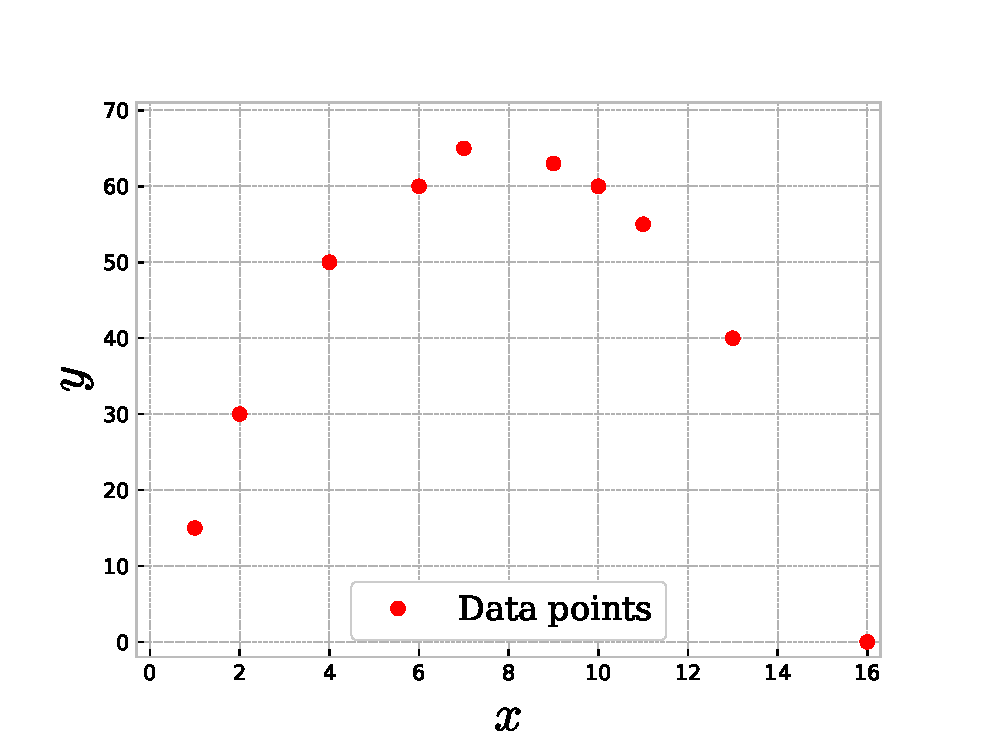
\includegraphics[width=8cm]{../Images/datapoints.eps}}}
	\subfloat[Data set with fitted polynomials]{{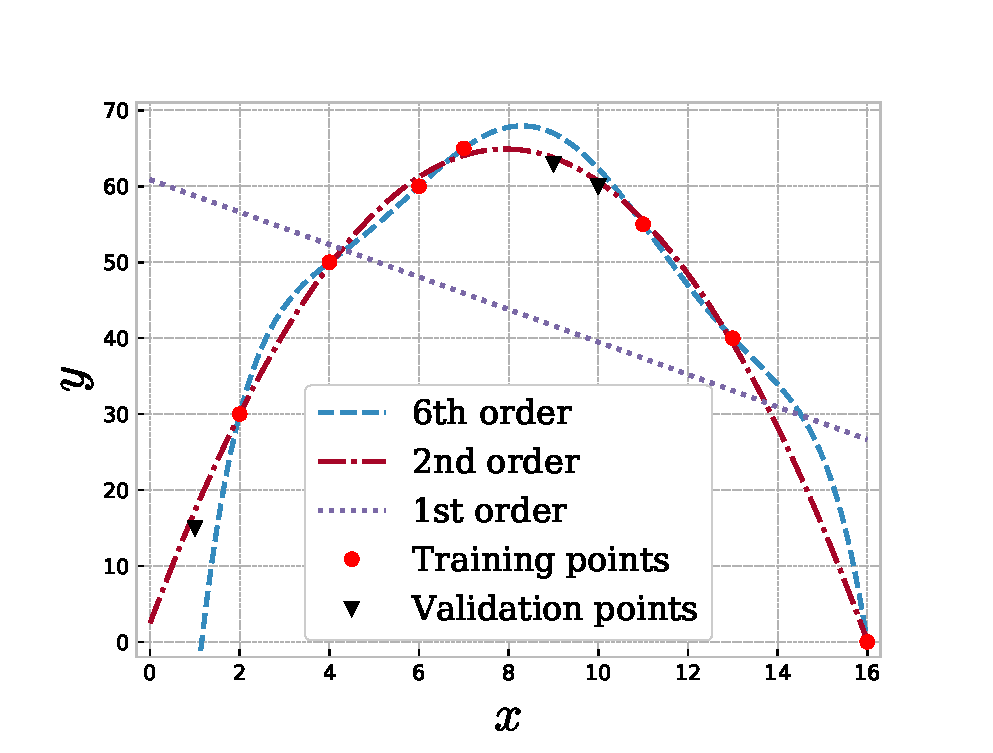
\includegraphics[width=8cm]{../Images/datacurve.eps} }}
	\caption{Figure (a) presents the data points given in equation \eqref{eq:datapoints}, while the figure (b) illustrates how a first-, second- and sixth order polynomial can be fitted to the training set in the best possible way.}%
	\label{fig:polynomials}
\end{figure}

\begin{table}
	\caption{Best fitting polynomials of first-, second- and sixth-order degree to the data set in equation \eqref{eq:datapoints}. $f(x)$ gives the actual form of the polynomial, the training error is the MSE of the training data set and the prediction error is the MSE of the validation data set.}
	\label{tab:example}
	\begin{tabularx}{\textwidth}{llR{6.5cm}R{3cm}R{3cm}} \hline\hline
		Order & \makecell{\\ \phantom{=}} & \multicolumn{1}{c}{$f(x)$} & Training error & Prediction error \\ \hline \\
		
		1st && $-2.14x+60.87$ & 327.22 & 927.87 \\
		2nd && $-x^2+15.74x + 2.51$ & 0.47 & 2.04 \\
		6th && $-0.001x^6+0.04x^5-0.90x^4+9.04x^3-47.52x^2+129.74x-98.67$ & 2.54E-11 & 187.53 \\ \hline\hline
	\end{tabularx}
\end{table}

What we immediately observe, is that the more complex model (higher degree polynomial), the lower the training error. The polynomial of sixth-order reproduces the points entirely. The first-order polynomial is quite bad, while the second-order polynomial is intermediate. However, what is most important is the prediction error as it shows the ability to reproduce data that is not prior known, and for that, we can see that the sixth-order polynomial performs terribly. When a model can reproduce the training set very well but is not able to reproduce the training set, we say that it overfits the data set. This means that the model is too complicated considering the problem. On the other hand, we see that the first-order polynomial also has a significant prediction error, which means that it is not able to reproduce the validation set either. We say that it is underfitted, and we are in need of a more complex model.

Finally, we have the second-order polynomial, which is miles ahead of its competitors when it comes to the prediction error. It turns out that the second-order model has an appropriate complexity, which we could have guessed just by looking at the data points. The natural question now is \textit{"How do we find a correct model complexity?"}. The answer is that there no easy way of doing this, which is one reason why machine learning is difficult. The trail and error method is the standard approach, where one examines various complexities and calculate the prediction error for each model. To find the prediction error precisely, one typically uses $K$ cross-validation resampling, which evaluates $K$ different choices of validation set to make the most use of the data. More about resampling analysis can be found in section \ref{sec:resampling}. A deeper understanding of the prediction error and how to reveal if a model overfits or under its will hopefully be gained in the next section, on bias-variance tradeoff. 

\section{Bias-variance tradeoff}
Up to this point, we have skipped some important terms in the statistics behind machine learning. First, we have the \textit{bias}, which describes the best our model could do if we had an infinite amount of training data. We also have the \textit{variance}, which is a measure of the fluctuations in the predictions. In figure (\ref{fig:bias_variance} a), an example of high variance low-bias and a low variance high bias models are presented. What we actually want is a low variance low-bias model, but this model is normally infeasible, and we need to find the optimal tradeoff between bias and variance. This is known as the bias-variance tradeoff. 

In figure (\ref{fig:bias_variance} b), the bias-variance tradeoff is illustrated as a function of the model complexity. We observe that the prediction error is large when the model complexity is too low, which corresponds to a low variance. This substantiates what we discussed in the example in section \ref{sec:example}, where we claimed that a too low model complexity under its data set. Therefore, a too low variance is associated with underfitting. On the other side of the plot, we can see that also a too complex model causes a large prediction error, which corresponds to a low bias. As discussed before, a too complex model overfits the model, which is associated with low bias. 

\begin{figure}
	\centering
	\subfloat[Illustration of bias and variance]{{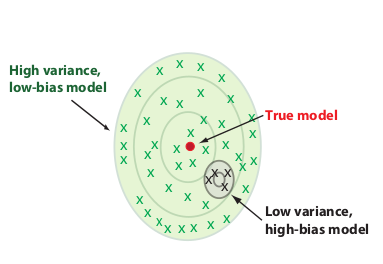
\includegraphics[width=8cm]{../Images/bias_variance.png}}}
	\subfloat[Bias-variance trade-off]{{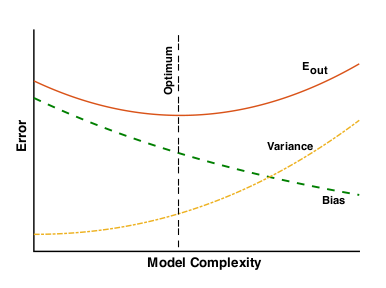
\includegraphics[width=8cm]{../Images/bias_variance_tradeoff.png} }}
	\caption{Examples of high variance, low-bias and low variance high-bias (a) and illustration of the bias-variance trade-off (b). Figures are taken from \citet{mehta_high-bias_2019}.}%
	\label{fig:bias_variance}
\end{figure}

To minimize the prediction error, we should therefore neither minimize the bias nor the variance. Instead, we should find the bias and variance which corresponds to the lowest error. To see how the error is distributed between the bias and variance, we can perform a so-called bias-variance decomposition. This is easiest if we assume that the true data is generated from a noisy model
\begin{equation}
y=f(x)+\epsilon
\end{equation}
where the noise, $\epsilon$, is normally distributed with mean zero and standard deviation $\sigma_{\epsilon}$. In that case, it can be shown that
\begin{equation}
\langle\langle(y_{\epsilon}-\tilde{y})^2\rangle\rangle_{\epsilon}=\underbrace{\sum_i(f(x_i)-\langle \tilde{y}\rangle)^2}_{\text{bias}^2}+\underbrace{\sum_i\langle(\tilde{y}-\langle \tilde{y}\rangle)^2\rangle}_{\text{variance}}+\underbrace{\sum_i\sigma_{\epsilon}^2}_{\text{noise}}
\end{equation}
where the expectation values are over the data set $\mathcal{D}$ if nothing else is specified. This decomposition is shown carefully by \citet{mehta_high-bias_2019}.

\section{Linear regression}
Polynomial regression, as already discussed, is an instance of linear regression and was meant as a motivation before we study linear regression in general. Instead of fitting a polynomial to a set of points, we can fit a general function in the form of
\begin{equation}
f(x_i)=\sum_{j=0}^pX_{ij}(x_i)\theta_j,
\label{eq:targets}
\end{equation}
where we have $p+1$ estimators $\theta_j$. The matrix $\bs{X}$ is called the \textit{design matrix}, and in the case where $X_{ij}(x_i)=x_i^j$ corresponds to polynomial regression, but it can in principle be an arbitrary function of $x_i$. The cost function for \textit{the ordinary least square regression} (OLS) case is already found in equation \eqref{eq:polynomialcost}, and we can recall it as
\begin{empheq}[box={\mybluebox[5pt]}]{equation}
\mathcal{C}(\bs{\theta})=\sum_{i=1}^{n}\Big(y_i-\sum_{j=0}^pX_{ij}\theta_j\Big)^2,\qquad\qquad\qquad\text{OLS}
\end{empheq}
which is minimized when
\begin{equation}
\bs{\theta}=(\bs{X}^T\bs{X})^{-1}\bs{X}^T\bs{y}.
\label{eq:ols}
\end{equation}

To solve this equation, we need to find the inverse of the matrix $\bs{X}^T\bs{X}$, which is typically done by \textit{lower-upper} (LU) decomposition or \textit{singular values decomposition} (SVD). However, quite often, when we deal with large data sets, the matrix above is singular, which means that the determinant of the matrix is zero. In those cases, we cannot find the inverse, and LU decomposition does not work. Fortunately, SVD \textit{always} works, and in cases where the matrix is singular, it turns out to be a good idea to perform such decomposition.

\subsection{Singular value decomposition}
Singular value decomposition is a method which decomposes an $m\times n$ matrix $\bs{X}$ into a product of three matrices, written as
\begin{equation}
\bs{X}=\bs{U}\bs{\Sigma}\bs{V}^T
\end{equation}
where $\bs{U}$ is a unitary $m\times m$ matrix, $\bs{V}$ is a unitary $n\times n$ matrix and $\bs{\Sigma}$ is a diagonal $m\times n$ matrix. This might sounds like a bad idea, but especially for singular matrices this often makes life easier. The reason for this, is that only $\bs{\Sigma}$ is singular after the decomposition. For our case, we can thus write the matrix $\bs{X}^T\bs{X}$ as 
\begin{equation}
\bs{X}^T\bs{X}=\bs{V}\bs{\Sigma}^T\bs{\Sigma}\bs{V}^T=\bs{V}\bs{D}\bs{V}^T
\end{equation}
where we exploit that $\bs{U}^T\bs{U}=\mathbb{1}$ and $\bs{\Sigma}^T\bs{\Sigma}=\bs{D}$ by definition. Further we can multiply by $\bs{V}$ on the right-hand-side
\begin{equation}
(\bs{X}^T\bs{X})\bs{V}=\bs{V}\bs{D}
\end{equation}
to get rid of the $\bs{V}^T$. A similar exercise can be done on $\bs{X}\bs{X}^T$, and we will obtain
\begin{equation}
(\bs{X}\bs{X}^T)\bs{U}=\bs{U}\bs{D}.
\end{equation}
By using the former of the two expressions, one can show that
\begin{equation}
\bs{X}\bs{\theta}=\bs{U}\bs{U}^T\bs{y}
\end{equation}
which is solvable even when $\bs{X}^T\bs{X}$ is singular.

\subsection{Ridge regression}
So, how can we avoid non-singular values in our matrix $\bs{X}^T\bs{X}$? We can remove them by introducing a penalty $\lambda$ to ensure that all the diagonal values are non-zero, which can be accomplished by adding a small value to all diagonal elements. By doing this, all diagonal elements will get a non-zero value and the matrix is guaranteed to be non-singular. Still using the matrix-vector form, this can be written as 
\begin{equation}
\bs{\theta}=(\bs{X}^T\bs{X}+\lambda\bs{I})^{-1}\bs{X}^T\bs{y}
\label{eq:ridgetheta}
\end{equation}
where $\bs{I}$ is the identity matrix. The penalty $\lambda$ is also a \textit{hyper-parameter}, which is a parameter that is specified before the training begins, in contrast to the estimators which are determined throughout training. This method is called Ridge regression, and has a cost function given by 
\begin{empheq}[box={\mybluebox[5pt]}]{equation}
\mathcal{C}(\bs{\theta})=\sum_{i=1}^{n}\Big(y_i-\sum_{j=0}^pX_{ij}\theta_j\Big)^2+\lambda\sum_{j=1}^p|\theta_j|^2,\qquad\text{Ridge}
\label{eq:ridge}
\end{empheq}
where we in principle just add the L2-norm of the estimator vector to the OLS cost function. The link between equation \eqref{eq:ridgetheta} and \eqref{eq:ridge} can be easiest found by going from the latter to the former, similarly to what we did for the polynomial regression in equations (\ref{eq:polynomialcost}-\ref{eq:polynomialestimators}).

\subsection{LASSO regression}
Finally, we introduce the \textit{least absolute shrinkage and selection operator} (LASSO) regression, which in the same way as Ridge regression is based on regularization. Instead of adding the L2-norm of the estimator matrix, we add the the L1-norm $|\theta_j|$, and the cost function expresses
\begin{empheq}[box={\mybluebox[5pt]}]{equation}
\mathcal{C}(\bs{\theta})=\sum_{i=1}^{n}\Big(y_i-\sum_{j=0}^pX_{ij}\theta_j\Big)^2+\lambda\sum_{j=1}^p|\theta_j|.\qquad\text{Lasso}
\end{empheq}
For LASSO regression, we cannot set $\partial\mathcal{C}(\bs{\theta})/\partial\theta_k=0$ and find a closed-form expression of $\bs{\theta}$, which means that we need to use an iterative optimization algorithm in order to obtain the optimal estimators. Such optimization methods are essential in non-linear problems such as deep neural networks and variational Monte Carlo. They will therefore be familiar to the reader throughout this thesis. In section \ref{sec:optimizationalgorithms}, we present various optimization methods, but from now on we will stick to one of the most basic methods, \textit{gradient descent}, which can be written as  
\begin{equation}
\theta_{k,t}=\theta_{k,t-1}-\eta \frac{\partial\mathcal{C}(\bs{\theta}_{t-1})}{\partial\theta_k},
\end{equation}
where $\theta_{k,t}$ is the parameter $\theta_k$ at iteration $t$ and $\mathcal{C}(\bs{\theta})$ is an arbitrary cost function. Here we are introduced to a new hyper-parameter, $\eta$, known as the \textit{learning rate}, which controls how much the estimators should be changed for each iteration. It has to be specified carefully, where a too large $\eta$ will make the cost function diverge and a too small $\eta$ will make the training too slow. Typically, to choose an $\eta\in[0.01-0.0001]$ is a good choice. For OLS, the vectorized iterative parameter update can be written as
\begin{equation}
\bs{\theta}_t=\bs{\theta}_{t-1}-\eta\bs{X}^T(\bs{y}-\bs{X}\bs{\theta}_{t-1}).
\label{eq:olsupdate}
\end{equation}

\section{Logistic regression}
So far, we have discussed polynomial regression and linear regression, which consist of models giving continuous outputs. However, what do we do if we want discrete outputs, for example, in the form of classification? This is what logistic regression is all about, where the name comes from the logistic function (sigmoid function) which is used to fire or not fire the neurons. As for the linear regression, we also need a cost function in logistic regression, which we will motivate in the following.

Consider a system that can take two possible energies $\varepsilon_0$ and $\varepsilon_1$. From elementary statistical mechanics, we know that the probability of finding a system in a state of a certain energy is given by the Boltzmann distribution, such that
\begin{align}
P(y_i=0)&=\frac{\exp(-\varepsilon_0/k_BT)}{\exp(-\varepsilon_0/k_BT)+\exp(-\varepsilon_1/k_BT)}\\
&=\frac{1}{1+\exp(-(\varepsilon_1-\varepsilon_0)/k_BT)},
\end{align}
which is the \textit{sigmoid function}, in the most general given by
\begin{equation}
f(x)=\frac{1}{1+\exp(-x)}.
\end{equation}
The first denominator is known as the \textit{partition function},
\begin{equation}
Z=\sum_{i=0}^1\exp(-\varepsilon_i/k_BT)
\label{eq:partition}
\end{equation}
where $k_B$ is Boltzmann's constant and $T$ is the system temperature. The probability of finding the system in the second state is given by
\begin{align}
P(y_i=1)&=1-P(y_i=0)\\
&=\frac{1}{1+\exp(-(\varepsilon_0-\varepsilon_1)/k_BT)}.
\end{align}
Notice that the only thing we need is the energy difference, $\Delta\varepsilon=\varepsilon_1-\varepsilon_0$, between the two states rather than the energy itself. This is often the case in physics, where we for instance have no absolute potential energy. If we now assume that the energy difference can be written as a function of the coordinates that specify the state $i$ stored in the row vector $\bs{X}_i$, and a column vector with parameters, $\bs{w}$, known as the \textit{weights}, the difference can be written as
\begin{figure}
	\centering
	\begin{tikzpicture}
\node[functions] (center) {};
\node[below of=center,text width=4em] {Activation function};
\draw[thick] (0.5em,0.5em) -- (0,0.5em) -- (0,-0.5em) -- (-0.5em,-0.5em);
\draw (0em,0.75em) -- (0em,-0.75em);
\draw (0.75em,0em) -- (-0.75em,0em);
\node[right of=center] (right) {};
\path[draw,->] (center) -- (right);
\node[functions,left=3em of center] (left) {$\sum$};
\path[draw,->] (left) -- (center);
\node[weights,left=3em of left] (2) {$w_2$} -- (2) node[input,left=2em of 2] (l2) {$X_{i2}$};
\path[draw,->] (l2) -- (2);
\path[draw,->] (2) -- (left);
\node[below of=2] (dots) {$\vdots$} -- (dots) node[left=2em of dots] (ldots) {$\vdots$};
\node[weights,below of=dots] (n) {$w_n$} -- (n) node[input,left=2em of n] (ln) {$X_{in}$};
\path[draw,->] (ln) -- (n);
\path[draw,->] (n) -- (left);
\node[weights,above of=2] (1) {$w_1$} -- (1) node[input,left=2em of 1] (l1) {$X_{i1}$};
\path[draw,->] (l1) -- (1);
\path[draw,->] (1) -- (left);
\node[weights,above of=1] (0) {$b$} -- (0) node[input,left=2em of 0] (l0) {$B$};
\node[right of=0] {bias};
\path[draw,->] (l0) -- (0);
\path[draw,->] (0) -- (left);
\node[below of=ln] {inputs};
\node[below of=n] {weights}; 
\end{tikzpicture}
	\caption{Logistic regression model with $n$ inputs. Each input $x_{j}$ is multiplied with a weight $w_j$, and the contributions from all units are summarized. The output is obtained after the sum is activated by an activation function.}
	\label{fig:single_perceptron}
\end{figure}
\begin{equation}
\Delta\varepsilon=\bs{X}_i\bs{w}\equiv\tilde{y}_i,
\end{equation}
giving the conditional probability
\begin{equation}
P(\bs{X}_i,y_i|\bs{w})=\big(f(\bs{X}_i\bs{w})\big)^{y_i}\big(1-f(\bs{X}_i\bs{w})\big)^{1-y_i}.
\end{equation}
If we have a set of multiple states stored in a  $\mathcal{D}=\{(\bs{X}_i,y_i)\}$, the joint probability yields
\begin{equation}
P(\mathcal{D}|\bs{w})=\prod_{i=1}^n\big(f(\bs{X}_i\bs{w})\big)^{y_i}\big(1-f(\bs{X}_i\bs{w})\big)^{1-y_i}
\end{equation}
which is known as the \textit{likelihood}. The \textit{log-likelihood} function is simply the log of the likelihood, and is given by 
\begin{equation}
l(\bs{w})=\sum_{i=1}^n\bigg[y_i\log f(\bs{X}_i\bs{w})+(1-y_i)\log(1-f(\bs{X}_i\bs{w}))\bigg].
\end{equation}
As in linear regression, we want to find a cost function which we can minimize in order to fit the model to the data set. Since the log-likelihood function is at its maximum at the highest probability, a natural choice is to set the cost function to the negative log-likelihood function,
\begin{equation}
\mathcal{C}(\bs{w})=-l(\bs{w})=-\sum_{i=1}^n\Big[y_i\log f(\bs{X}_i\bs{w})+(1-y_i)\log(1-f(\bs{X}_i\bs{w}))\Big],
\end{equation}
which is the \textit{cross entropy}. To clarify things, we will try to illustrate how this works. In figure (\ref{fig:single_perceptron}), we have an input set $\bs{X}_i$ where each unit is multiplied with a parameter from $\bs{w}$ and summarized. This corresponds to the inner product $\bs{X}_i\bs{w}$. Further, the sum (or the inner product) is \textit{activated} by an \textit{activation function}, which we above have assumed to be the sigmoid function. The output is then given by
\begin{eqnarray}
a_i=f(\bs{X}_i\bs{w}),
\end{eqnarray}
where the bias node is included in the $\bs{X}_i$'s and the bias weights are included in the $\bs{w}$'s. The bias node is added in order to shift the activation function to the left or right, and works in the same way as a constant term in a function. 

The output from the activation is used further in the cost function to calculate the cost. As for LASSO regression, the cost function is then minimized in an iterative scheme, where for example the gradient descent method gives the weight update
\begin{empheq}[box={\mybluebox[5pt]}]{align}
\bs{w}_t= \bs{w}_{t-1} - \eta\bs{X}[\bs{y}-f(\bs{X}\bs{w}_{t-1})]
\end{empheq}
where $\bs{X}$ is a matrix containing all the column vectors $\bs{X}_i$. This expression is extremely similar, not to say identical to the estimator update for ordinary least square presented in equation \eqref{eq:olsupdate}. The difference is that we now denote the parameters by $\bs{w}$ instead of $\bs{\theta}$ to prepare for the neural networks, but they are basically the same thing. 

\section{Neural networks} \label{sec:neural_network}
Now we know enough to dive into the field of artificial neural networks. Neural networks can give either continuous or discrete outputs and are therefore, competitors to both linear and logistic regression. The great strength of neural networks is that one can add multiple \textit{layers}, which potentially makes the model extremely flexible. According to \textbf{the universal approximation theorem}, a neural network with only one hidden layer with a finite number of units can approximate any continuous function \cite{hornik_multilayer_1989}. However, often, multiple layers are used since those networks are in general known to be easier to train and work better for complex systems. Neural networks of more than one layer are called \textit{deep} networks, and as more layers are added, the network gets \textit{deeper}.

In figure \eqref{fig:neural_network}, we have illustrated a deep neural network with an unspecified number of layers and five hidden units in each layer. It has some similarities with the logistic regression model in figure \eqref{fig:single_perceptron}, but with multiple hidden layers and multiple outputs, this model is more complicated. We decided to drop the representation of the weights (apart from some selected labeled ones), but each line corresponds to a weight.

Without a hidden layer, we have seen that the update of weights is quite straight forward. For a neural network consisting of multiple layers, the question is: \textit{How do we update the weights when we do not know the values of the hidden units?} This will be explained in section \ref{sec:backward}, where backward propagation, the most popular technique for weight update in a neural network, is discussed. Before that, we will generalize the forward phase presented in logistic regression.

\begin{figure}
	\centering
	\begin{tikzpicture}

% Define outputs
\node[] (center) {};
\node[input, above=0.3em of center] (y1) {$y_1$};
\node[input, below=0.3em of center] (y2) {$y_2$};

% Draw lines from output nodes
\node[right of=y1] (righty1) {};
\node[right of=y2] (righty2) {};
\path[draw,->] (y1) -- (righty1);
\path[draw,->] (y2) -- (righty2);

% Hidden nodes L
\node[input,left=5em of center] (aL3) {$a_3^{(L)}$};
\node[input,above of=aL3] (aL2) {$a_2^{(L)}$};
\node[input,above of=aL2] (aL1) {$a_1^{(L)}$};
\node[input,below of=aL3] (aL4) {$a_4^{(L)}$};
\node[input,below of=aL4] (aL5) {$a_5^{(L)}$};
\node[input,above of=aL1] (bL) {$B_L$};

% Hidden nodes 1
\node[input,left=25em of center] (a13) {$a_3^{(1)}$};
\node[input,above of=a13] (a12) {$a_2^{(1)}$};
\node[input,above of=a12] (a11) {$a_1^{(1)}$};
\node[input,below of=a13] (a14) {$a_4^{(1)}$};
\node[input,below of=a14] (a15) {$a_5^{(1)}$};
\node[input,above of=a11] (b1) {$B_1$};

% Hidden nodes l
\node[input,left=15em of center] (al3) {$a_3^{(l)}$};
\node[input,above of=al3] (al2) {$a_2^{(l)}$};
\node[input,above of=al2] (al1) {$a_1^{(l)}$};
\node[input,below of=al3] (al4) {$a_4^{(l)}$};
\node[input,below of=al4] (al5) {$a_5^{(l)}$};
\node[input,above of=al1] (bl) {$B_l$};

% Draw lines from hidden nodes
\path[draw,->] (aL1) -- (y1);
\path[draw,->] (aL2) -- (y1);
\path[draw,->] (aL3) -- (y1);
\path[draw,->] (aL4) -- (y1);
\path[draw,->] (aL5) -- (y1);
\path[draw,->] (bL) -- (y1);

\path[draw,->] (aL1) -- (y2);
\path[draw,->] (aL2) -- (y2);
\path[draw,->] (aL3) -- (y2);
\path[draw,->] (aL4) -- (y2);
\path[draw,->] (aL5) -- (y2) node[midway,below] {$w_{52}^{(L+1)}$};
\path[draw,->] (bL) -- (y2);

% Define place left of left
\node[input,left=5em of a13] (x2) {$x_2$};
\node[input,above of=x2] (x1) {$x_1$};
\node[input,below of=x2] (x3) {$x_3$};
\node[input,above of=x1] (b0) {$B_0$};

% Draw lines from input nodes
\path[draw,->] (x1) -- (a11);
\path[draw,->] (x1) -- (a12);
\path[draw,->] (x1) -- (a13);
\path[draw,->] (x1) -- (a14);
\path[draw,->] (x1) -- (a15);

\path[draw,->] (x2) -- (a11);
\path[draw,->] (x2) -- (a12);
\path[draw,->] (x2) -- (a13);
\path[draw,->] (x2) -- (a14);
\path[draw,->] (x2) -- (a15);

\path[draw,->] (x3) -- (a11);
\path[draw,->] (x3) -- (a12);
\path[draw,->] (x3) -- (a13);
\path[draw,->] (x3) -- (a14);
\path[draw,->] (x3) -- (a15) node[midway,below] {$w_{35}^{(1)}$};

\path[draw,->] (b0) -- (a11);
\path[draw,->] (b0) -- (a12);
\path[draw,->] (b0) -- (a13);
\path[draw,->] (b0) -- (a14);
\path[draw,->] (b0) -- (a15);

% Draw lines from first hidden layer
\path[draw,dashed,->] (a11) -- (al1);
\path[draw,dashed,->] (a11) -- (al2);
\path[draw,dashed,->] (a11) -- (al3);
\path[draw,dashed,->] (a11) -- (al4);
\path[draw,dashed,->] (a11) -- (al5);

\path[draw,dashed,->] (a12) -- (al1);
\path[draw,dashed,->] (a12) -- (al2);
\path[draw,dashed,->] (a12) -- (al3);
\path[draw,dashed,->] (a12) -- (al4);
\path[draw,dashed,->] (a12) -- (al5);

\path[draw,dashed,->] (a13) -- (al1);
\path[draw,dashed,->] (a13) -- (al2);
\path[draw,dashed,->] (a13) -- (al3);
\path[draw,dashed,->] (a13) -- (al4);
\path[draw,dashed,->] (a13) -- (al5);

\path[draw,dashed,->] (a14) -- (al1);
\path[draw,dashed,->] (a14) -- (al2);
\path[draw,dashed,->] (a14) -- (al3);
\path[draw,dashed,->] (a14) -- (al4);
\path[draw,dashed,->] (a14) -- (al5);

\path[draw,dashed,->] (a15) -- (al1);
\path[draw,dashed,->] (a15) -- (al2);
\path[draw,dashed,->] (a15) -- (al3);
\path[draw,dashed,->] (a15) -- (al4);
\path[draw,dashed,->] (a15) -- (al5) node[midway,below] {$w_{55}^{(l)}$};

\path[draw,dashed,->] (b1) -- (al1);
\path[draw,dashed,->] (b1) -- (al2);
\path[draw,dashed,->] (b1) -- (al3);
\path[draw,dashed,->] (b1) -- (al4);
\path[draw,dashed,->] (b1) -- (al5);

% Draw lines to last hidden layer
\path[draw,dashed,->] (al1) -- (aL1);
\path[draw,dashed,->] (al1) -- (aL2);
\path[draw,dashed,->] (al1) -- (aL3);
\path[draw,dashed,->] (al1) -- (aL4);
\path[draw,dashed,->] (al1) -- (aL5);

\path[draw,dashed,->] (al2) -- (aL1);
\path[draw,dashed,->] (al2) -- (aL2);
\path[draw,dashed,->] (al2) -- (aL3);
\path[draw,dashed,->] (al2) -- (aL4);
\path[draw,dashed,->] (al2) -- (aL5);

\path[draw,dashed,->] (al3) -- (aL1);
\path[draw,dashed,->] (al3) -- (aL2);
\path[draw,dashed,->] (al3) -- (aL3);
\path[draw,dashed,->] (al3) -- (aL4);
\path[draw,dashed,->] (al3) -- (aL5);

\path[draw,dashed,->] (al4) -- (aL1);
\path[draw,dashed,->] (al4) -- (aL2);
\path[draw,dashed,->] (al4) -- (aL3);
\path[draw,dashed,->] (al4) -- (aL4);
\path[draw,dashed,->] (al4) -- (aL5);

\path[draw,dashed,->] (al5) -- (aL1);
\path[draw,dashed,->] (al5) -- (aL2);
\path[draw,dashed,->] (al5) -- (aL3);
\path[draw,dashed,->] (al5) -- (aL4);
\path[draw,dashed,->] (al5) -- (aL5) node[midway,below] {$w_{55}^{(L)}$};

\path[draw,dashed,->] (bl) -- (aL1);
\path[draw,dashed,->] (bl) -- (aL2);
\path[draw,dashed,->] (bl) -- (aL3);
\path[draw,dashed,->] (bl) -- (aL4);
\path[draw,dashed,->] (bl) -- (aL5);

% Draw lines towards input nodes
\node[left of=x1] (leftx1) {};
\node[left of=x2] (leftx2) {};
\node[left of=x3] (leftx3) {};
\path[draw,->] (leftx1) -- (x1);
\path[draw,->] (leftx2) -- (x2);
\path[draw,->] (leftx3) -- (x3); 

% Add some text
\node[below=6.1em of x2] {input};
\node[below=6em of a13] {hidden 1};
\node[below=6em of al3] {hidden l};
\node[below=6em of aL3] {hidden L};
\node[below=6.8em of center] {output};
\end{tikzpicture}
	\caption{Neural network with 3 input units, $L$ hidden layers with 5 hidden units each and two outputs. $B^{(0)}$, $B^{(1)}$, $B^{(l)}$ and $B^{(L)}$ are the bias units for the respective layers, and the dashed lines indicate that it might be more layers between the two layers. We have labeled a few of the lines to relate them to the weights.}
	\label{fig:neural_network}
\end{figure}

\subsection{Forward phase}
In the previous section, we saw how the output is found for a single perceptron. For a neural network, the net output to the first layer is similar, and given by
\begin{equation*}
z_j^{(1)}=\sum_{i=1}^{N_0}x_iw_{ij}^{(0)}=\bs{X}\bs{w}_j^{(0)}
\end{equation*}
where $N_0$ is the number of units in layer 0 (the input layer), $\bs{X}$ is the input vector which is assumed to be a row vector and $\bs{w}_j^{(1)}$ is the $i$'th column of the $\bs{w}$-matrix associated with the first layer. We have again assumed that the bias node is included in $\bs{X}$ and the first set of bias weights are included in $\bs{w}^{(1)}$. The same applies for the other layers as well. If we let the activation function, $f(x)$, act on the net output, we get the real output given by
\begin{equation*}
a_j^{(1)}=f(z_j^{(1)})=f\Big(\sum_{i=1}^{N_0}x_iw_{ij}^{(0)}\Big).
\end{equation*}
This is then again the input to the next layer with $N_1$ units, so the output from the second layer is simply
\begin{equation*}
a_j^{(2)}=f\Big(\sum_{i=1}^{N_1}a_i^{(1)}w_{ij}^{(1)}\Big).
\end{equation*}
For a neural network of multiple layers, the same procedure applies for all the layers and we can find a general formula for the output at a layer $l+1$. The net output to a node $z_j^{(l+1)}$ in layer $l+1$ can be found to be
\begin{empheq}[box={\mybluebox[5pt]}]{equation}
z_j^{(l+1)}=\sum_{i=1}^{N_{l}}a_i^{(l)}w_{ij}^{(l)}
\label{eq:netoutput}
\end{empheq}
where layer $l$ has $N_{l}$ units and we need to be aware that $a_j^{(0)}=x_j$. After activation, the output is obviously found to be
\begin{empheq}[box={\mybluebox[5pt]}]{equation}
a_j^{(l+1)}=f(z_j^{(l+1)})=f\Big(\sum_{i=1}^{N_{l}}a_i^{(l)}w_{ij}^{(l)}\Big)
\label{eq:output}
\end{empheq}
which is the only formula needed for the forward phase. In practice, the operation is always implemented in a vectorized fashion, reading $\bs{a}^{(l+1)}=f(\bs{a}^{(l)}\bs{w}^{(l)})$. The activation function $f(x)$ is not explicitly defined, because it is often expedient having the chance to experiment with multiple activation functions. 

\subsection{Activation function}
The task of the activation function is to define the output from a unit given an input. There are multiple reasons to do this, where the most important include filter the intensity of the output and make the output non-linear. Without an activation function, all of our layers would simply stack one affine transformation after another, resulting in a composition of transformations equal to such transformation. In other words, the deep networks would have lost their clout without the activation functions. 

Yet, we have only discussed the sigmoid activation function, but there plenty of other activation functions available. The sigmoid function has lost its popularity, and is today superseded by the more advanced functions based on \textit{rectified linear units} (ReLU). Some popular choices are the \textit{leaky} ReLU and \textit{exponential linear units} (ELU), which are linear for positive numbers. The pure linear activation function is still widely used, especially on the output layer. In figure (\ref{fig:activation_functions}), standard RELU, leaky RELU and ELU are plotted along with the sigmoid function.

\begin{figure}
	\centering
	\subfloat{{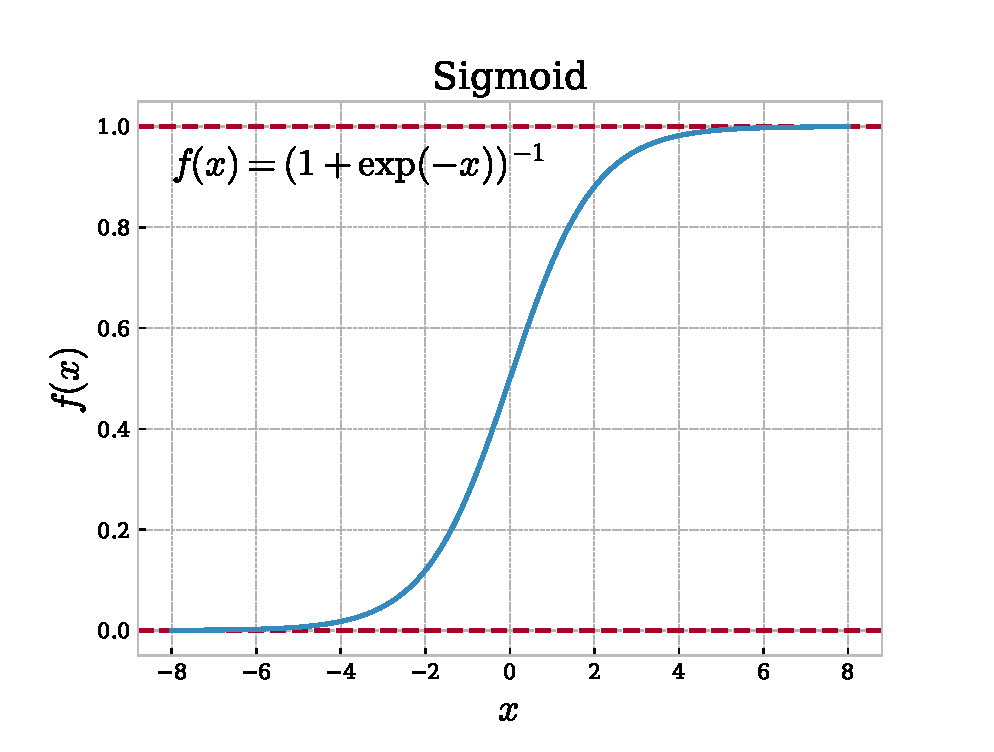
\includegraphics[width=7cm]{../Images/sigmoid.eps}}}
	\subfloat{{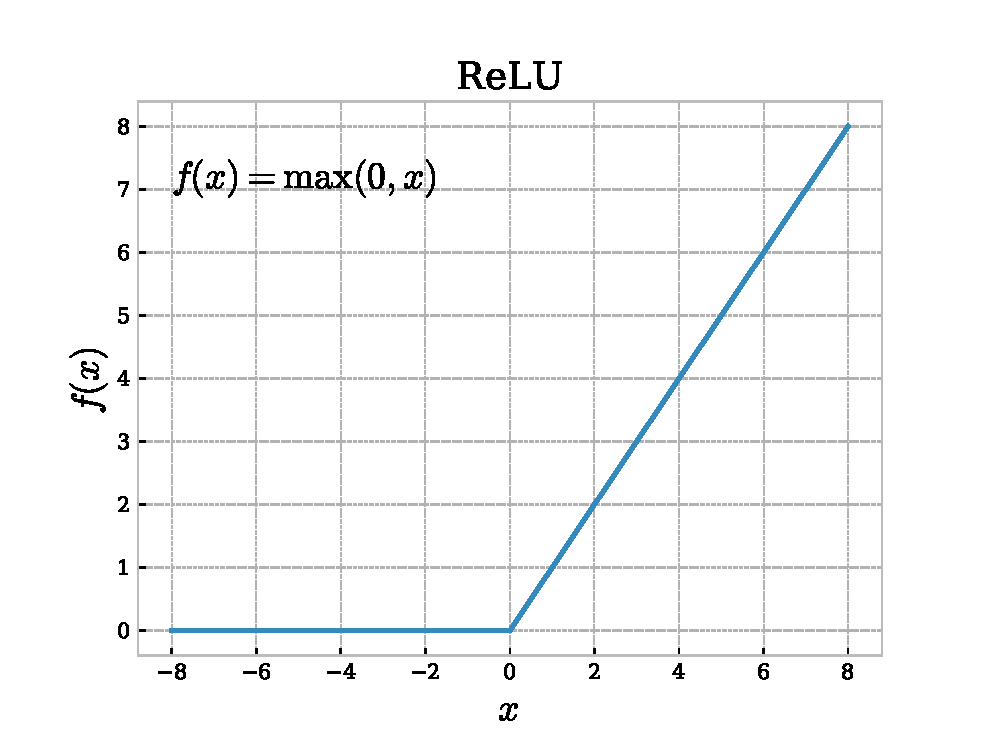
\includegraphics[width=7cm]{../Images/ReLU.eps}}}\\
	
	\subfloat{{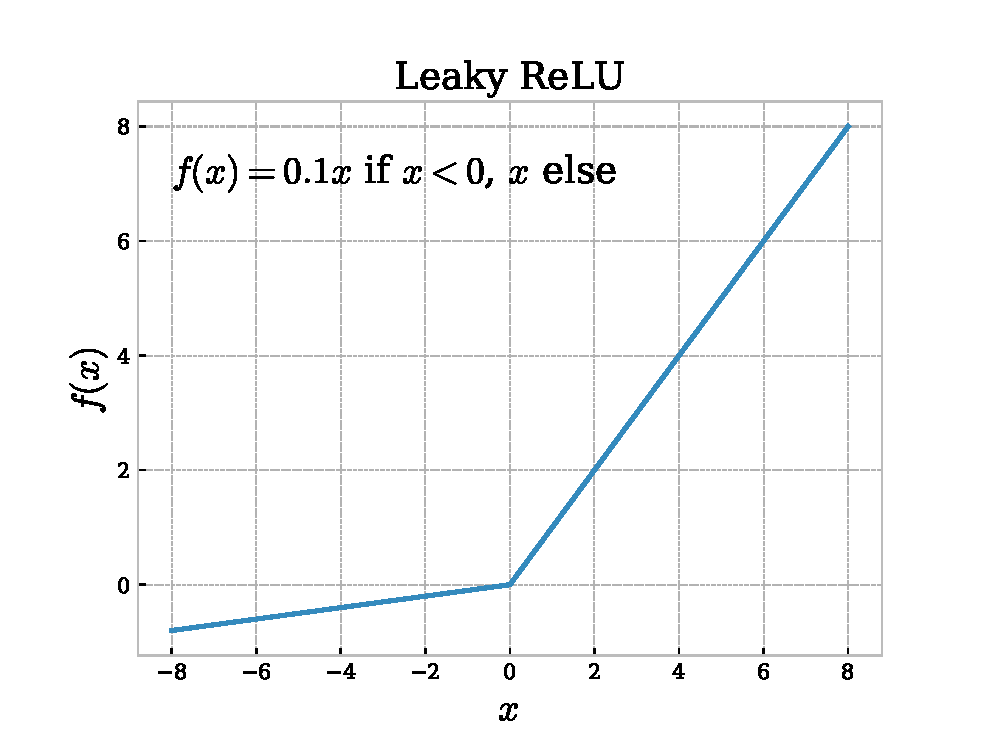
\includegraphics[width=7cm]{../Images/LeakyReLU.eps}}}
	\subfloat{{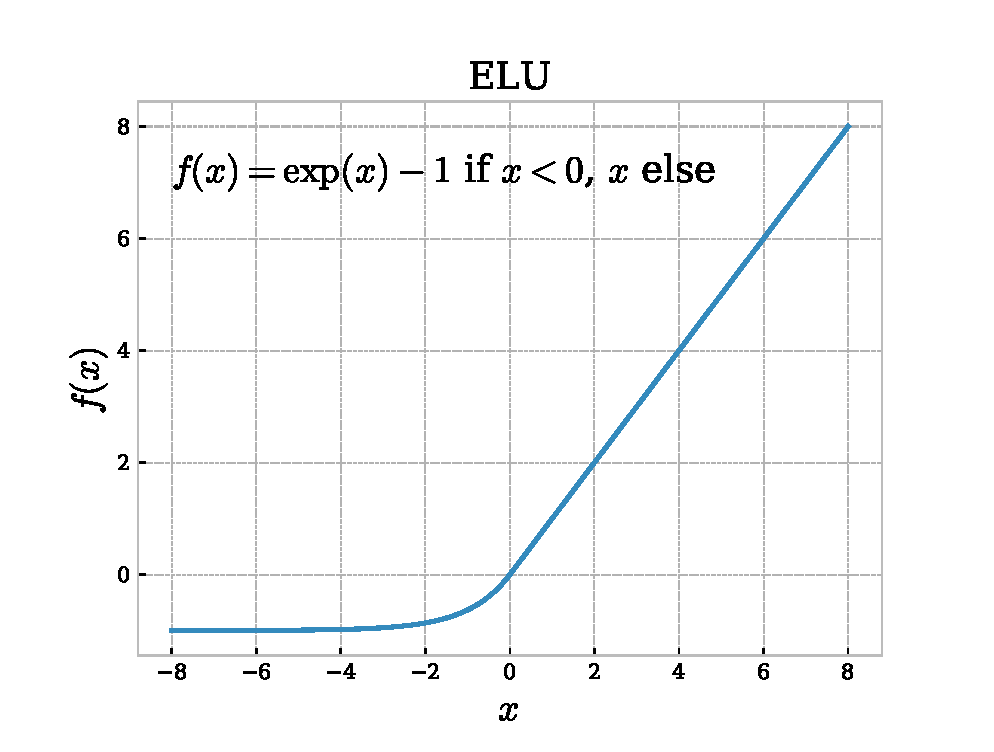
\includegraphics[width=7cm]{../Images/ELU.eps}}}
	\caption{Some well-known activation functions. The sigmoid function stands out from the others since it maps between 0 and 1, and it is not linear for positive numbers.}%
	\label{fig:activation_functions}%
\end{figure}


\subsection{Backward propagation} \label{sec:backward}
Backward propagation is the most robust technique for updating the weights in a neural network and is again based on the weight update presented for linear and logistic regression. The algorithm for this was presented in 1986, which made the deep neural networks able to solve relatively complicated problems for the first time \cite{rumelhart_learning_1986}. To update the weights, one starts with the outputs and updates the weights layer-wise until one gets to the inputs, hence the backward propagation name. 

As observed above, a unit is dependent on all the units in the previous layers, and so are the weights. This means that the units are dependent on a large number of parameters, which makes the training scheme quite complex. Nevertheless, it is possible to generalize this to express the updating formulas on a relatively simple form, like the forward phase. From the linear and logistic regression, we know that we need the derivative of the cost function in order to implement the weight update regime. Again, we define the cost function as the mean square error,
\begin{equation}
\mathcal{C}(\bs{w})=\frac{1}{2}\sum_{i=1}^{N_L}(y_i-a_i^{(L+1)})^2,
\end{equation}
where we have $L$ hidden layers ($L+1$ is the last layer) and $N_{L+1}$ output units. The derivative of this with respect to one of the weights between the $L$'th and $L+1$'th layer can be written as a sum using the chain rule
\begin{equation}
\frac{\partial\mathcal{C}(\bs{w})}{\partial w_{jk}^{(L)}}=\frac{\partial\mathcal{C}(\bs{w})}{\partial a_j^{(L+1)}}\frac{\partial a_j^{(L+1)}}{\partial z_j^{(L+1)}}\frac{\partial z_j^{(L+1)}}{\partial w_{jk}^{(L)}}.
\end{equation}
where $z_j^{(L+1)}$ and $a_j^{(L+1)}$ are found from equations \eqref{eq:netoutput} and \eqref{eq:output} respectively. If we start with the first factor, it can easily be obtained as
\begin{equation}
\frac{\partial\mathcal{C}(\bs{w})}{\partial a_j^{(L+1)}}=-(y_j-a_j^{(L+1)})
\end{equation}
using the definition of the cost function. The second factor is the derivative of the activation function with respect to its argument, and is for the sigmoid function given by
\begin{equation}
\frac{\partial a_j^{(L+1)}}{\partial z_j^{(L+1)}}=a_j^{(L+1)}(1-a_j^{(L+1)}).
\end{equation}
Finally, the last factor is found from equation \eqref{eq:netoutput}, and we obtain
\begin{equation}
\frac{\partial z_j^{(L+1)}}{\partial w_{jk}^{(L)}}=a_k^{(L)}.
\end{equation}
Collecting all the factors, the update of the last set of weights can be found by
\begin{equation}
\frac{\partial\mathcal{C}(\bs{w})}{\partial w_{jk}^{(L)}}=-(y_j-a_j^{(L+1)})a_j^{(L+1)}(1-a_j^{(L+1)})a_k^{(L)}
\end{equation}
when the sigmoid function is used in the activation. In the next step, we can define
\begin{equation}
\delta_j^{(L+1)}=-a_j^{(L+1)}(1-a_j^{(L+1)})(y_j-a_j^{(L+1)})=f'(a_j^{(L+1)})\frac{\partial \mathcal{C}(\bs{w})}{\partial a_j^{(L+1)}}=\frac{\partial \mathcal{C}(\bs{w})}{\partial z_j^{(L+1)}}
\end{equation}
such that the weight update can be expressed on a neater form
\begin{equation}
\frac{\partial\mathcal{C}(\bs{w})}{\partial w_{jk}^{(L)}}=\delta_j^{(L+1)}a_k^{(L)}.
\end{equation}

For a general layer $l$, the derivative of the cost function with respect to a weight $w_{jk}^{(l)}$ is similar, and given by
\begin{empheq}[box={\mybluebox[5pt]}]{equation}
\frac{\partial\mathcal{C}(\bs{w})}{\partial w_{jk}^{(l)}}=\delta_j^{(l+1)}a_k^{(l)}.
\end{empheq}
Our goal is to find the general relation between layer $l$ and $l+1$, and therefore we use the chain rule and sum over all the net outputs in layer $l+1$,
\begin{equation}
\delta_j^{(l)}=\frac{\partial \mathcal{C}(\bs{w})}{\partial z_j^{(l)}}=\sum_k\frac{\partial\mathcal{C}(\bs{w})}{\partial z_k^{(l+1)}}\frac{\partial z_k^{(l+1)}}{\partial z_j^{(l)}}.
\end{equation}
We now recognize that the first factor in the sum is just $\delta_k^{(l+1)}$ and the last factor can be found from equation \eqref{eq:netoutput}. We obtain the final expression, 
\begin{empheq}[box={\mybluebox[5pt]}]{equation}
\delta_j^{(l)}=\sum_k\delta_k^{(l+1)}w_{kj}^{(l)}f'(z_j^{(l)}),
\end{empheq}
where we use the expression of $\delta_j^{(L)}$ as our initial condition. As for several of the methods discussed above, a solution of the weight update does not exist in closed form and we need to rely on iterative optimization methods. Using gradient descent, a new set of weights $\bs{w}_t$ is found from
\begin{equation}
\bs{w}_t=\bs{w}_{t-1}-\eta\frac{\partial\mathcal{C}(\bs{w}_{t-1})}{\partial \bs{w}_{t-1}},
\end{equation}
where the multi-dimensional differentiation is done element-wise. Other optimization methods will be discussed in the following section.

\section{Optimization algorithms} \label{sec:optimizationalgorithms}
We have above discussed the gradient descent optimization algorithm, which is among the most basic optimization methods available. That method is based on the gradient, which is the slope of the cost function. However, many other methods are also in need of the Hessian matrix, which gives the curvature of the cost function. We will barely scratch the surface of this field, limiting us to the gradient methods. 

To have the method fresh in mind, we will start with reintroducing the gradient descent method before we move on to its stochastic brother. We will then take a look at how momentum can be added, and finally, we examine the stochastic and momentum-based ADAM optimizer. Given a cost function $\mathcal{C}(\bs{\theta})$, the gradient with respect to a parameter $\theta$ can be found from
\begin{equation}
\nabla_{\theta} \mathcal{C}(\bs{\theta})\equiv\frac{\partial \mathcal{C}(\bs{\theta})}{\partial \bs{\theta}},
\end{equation}
where we henceforth use the short-hand notation with $\nabla_{\theta}$ representing the multi-dimensional derivative $\partial/\partial\bs{\theta}$. Differentiating with respect to the vector implies that the operation shall be done element-wise.

\subsection{Gradient descent} \label{sec:gd}
Perhaps the simplest and most intuitive method for finding the minimum is the gradient descent method, which reads
\begin{empheq}[box={\mybluebox[5pt]}]{align}
\label{eq:GD}
\bs{\theta}_t=\bs{\theta}_{t-1} - \eta\nabla_{\theta} \mathcal{C}(\bs{\theta}_{t-1})
\end{empheq}
where $\bs{\theta}_t$ is the parameter vector at time step (iteration) $t$ and $\eta$ is the learning rate. $\nabla_{\theta} \mathcal{C}(\bs{\theta}_{t-1})$ is the gradient of the cost function with respect to all the parameters $\theta$ at time $t-1$. 

The idea is to find the direction where the cost function $\mathcal{C}(\bs{\theta})$ has the steepest slope, and move in the direction which minimizes the cost function. For every time step, the cost function is thus minimized, and when the gradient approaches zero, the minimum is found. A possible, but basic, stop criterion is
\begin{equation}
\nabla_{\theta} \mathcal{C}(\bs{\theta}_t)<\epsilon
\end{equation}
where $\epsilon$ is a tolerance. More robust methods are based on comparing the value of the cost function for several past iterations. In cases where the cost function is not strictly decreasing, we will have both local and global minima. Often, it is hard to say whether we are stuck in a local or global minimum, and this is where the stochasticity enters the game.

\subsection{Stochastic gradient descent}\label{sec:sgd}
Stochastic gradient descent is closely related to the gradient descent method, but the method uses randomly selected batches to evaluate the gradients, hence the stochasticity. By introducing this randomness, the parameters will not always be updated in order to minimize the energy, which makes us less likely to be stuck in a local minimum.

In practice, one splits the data set in $n$ batches, and select one of them to be used in the parameter update. Our hope is that this batch is representative of the entire data set, such that the new parameters provide a lower cost function. If that is the case, we have reduced the cost of an iteration significantly, since we only need to care about a batch. We are not guaranteed that updating the parameters with respect to a batch gives a lower cost function, and when it is not, we need to run more batches in order to minimize the cost function. Since each iteration is faster than for standard gradient descent, this is acceptable. As long as the batch is slightly representative of the entire data set, the cost function will be minimized in the end. After each batch in the data set has had an opportunity to update the internal parameters, we say that we have gone through an \textit{epoch}. Mathematically, the method can be expressed as 
\begin{empheq}[box={\mybluebox[5pt]}]{align}
\label{eq:SGD}
\bs{\theta}_t=\bs{\theta}_{t-1} - \eta\nabla_{\theta} \mathcal{C}_i(\bs{\theta}_{t-1}),
\end{empheq}
where we use the $i$'th batch in the parameter update. Standard gradient descent is just a special case of this, where we only have one batch ($i$ includes the whole data set). If we still get stuck in local minima after adding the stochasticity, it might be a good idea to add momentum as well.

\subsection{Adding momentum} \label{sec:momentum}
If we now recall what we learned in an introductory mechanics course, we might remember that momentum is a quantity that maintains the motion of a body. Imagine a ball that rolls down a steep hill, but then there is a local minimum that it needs to escape to keep rolling. If it has enough momentum, it will be able to escape.

The same idea lies behind the momentum used in optimization algorithms; the momentum will try to maintain the motion towards the global minimum, which makes the system less likely to be stuck in a local minimum. Momentum can be added to most optimization algorithms, also gradient descent and stochastic gradient descent. The way we do it is to save the direction we were moving during the previous iteration, and use it as a contribution to the next gradient update. A typical implementation of the first-order momentum applied on gradient descent looks like
\begin{empheq}[box={\mybluebox[5pt]}]{equation}
\begin{aligned}
\bs{m}_t &= \gamma\bs{m}_{t-1} + \eta\nabla_{\theta} \mathcal{C}_i(\bs{\theta}_{t-1})\\
\bs{\theta}_t&=\bs{\theta}_{t-1}-\bs{m}_t
\end{aligned}
\end{empheq}
where $\gamma$ is the momentum parameter, which is just another hyper-parameter usually initialized to a small number. $\bs{m}_t$ is the momentum vector and can be initialized as the zero vector, corresponding to no initial momentum.

\IncMargin{1em}
\begin{algorithm}
	\SetAlgoLined
	\Parameter{$\eta$: Learning rate}
	\Parameter{$\gamma$: Momentum parameter}
	\Parameter{$\lambda$: Monotonic decay rate}
	\Require{$\mathcal{C}(\bs{\theta})$: Cost function}
	\Data{$\bs{\theta}_0$: Initial parameters}
	
	$\bs{m}_0\leftarrow 0$ (Initialize momentum vector)\;
	$t\leftarrow 0$ (Initialize time step)\;
	\While{$\bs{\theta}_t$ not converged}{
		$t\leftarrow t+1$ (Increase time for each iteration)\;
		$\bs{g}_t\leftarrow \nabla_{\theta}\mathcal{C}_t(\bs{\theta}_{t-1})$ (Get gradients from a given batch at time $t$)\;
		$\bs{m}_t\leftarrow \gamma\bs{m}_{t-1}+\eta\cdot\bs{g}_t$ (Update first momentum estimate)\;
		$\bs{\theta}_t=\bs{\theta}_{t-1}-\bs{m}_t/\lambda^t$ (Update parameters with monotonic, adaptive step)\;
	}
	\KwResult{Converged parameters $\bs{\theta}_t$.}
	\caption{Adaptive stochastic gradient descent with momentum. See sections (\ref{sec:sgd}-\ref{sec:momentum}) for details. Robust default settings for the hyper-parameters are $\eta=0.001$, $\gamma=0.01$ and $\lambda=0.1$. All the operations are element-wise.}
	\label{alg:asgd}
\end{algorithm}\DecMargin{1em}

The optimization algorithm can be modified further in unlimited ways. A common improvement is to add higher-order momentum; another is to make the learning-rate adaptive. We have implemented the most basic version of this, with monotonic adaptivity. Many algorithms, such as the conjugate gradient method, also make use of the Hessian as discussed in the introductory word to this section, but that is another level of complexity. We will end this section by setting up the algorithm of a stochastic gradient descent optimization with momentum and monotonic adaptivity. The algorithm is found in algorithm \ref{alg:asgd}.

\subsection{ADAM} \label{sec:adam}
ADAM is a first-order stochastic optimization method which is widely used in machine learning. It was discovered by \citet{kingma_adam:_2014}, and published in a 2014 paper. The article has already more than 30,000 citations! So what makes this method so popular? 

The main reason why it is widely used, is obviously that it provides good performance. The fact that it only requires the gradient makes it efficient, and the way the momentum is implemented still makes it capable of handle a large number of parameters. The optimization algorithm can be expressed as a set of equations
\begin{empheq}[box={\mybluebox[5pt]}]{equation}
\begin{aligned}
\bs{g}_t&=\nabla_{\theta} \mathcal{C}_t(\bs{\theta}_{t-1})\\
\bs{m}_t&=\gamma_1\bs{m}_{t-1}+(1-\gamma_1)\bs{g}_t\\
\bs{v}_t&=\gamma_2\bs{v}_{t-1}+(1-\gamma_2)\bs{g}_t^2\\
\hat{\bs{m}}_t&=\bs{m}_t/(1-\gamma_1^t)\\
\hat{\bs{v}}_t&=\bs{v}_t/(1-\gamma_2^t)\\
\bs{\theta}_t&=\bs{\theta}_{t-1}-\eta\hat{\bs{m}}_t/(\sqrt{\hat{\bs{v}}_t}+\bs{\varepsilon})
\end{aligned}
\end{empheq}
where $\bs{m}_t$ is the biased first momentum estimate of the parameter vector $\bs{\theta}$ and $\bs{v}_t$ is the biased second raw moment estimate. The momentum parameters need to be in the range $\gamma_1,\gamma_2\in[0,1)$, and are often set to values close to 1. This makes the optimization adaptive, as the time goes the factors $1-\gamma_1^t$ and $1-\gamma_2^t$ approach 1 from below. $\eta$ is the learning rate, and should be a small number. Finally, the parameters $\bs{\varepsilon}$ are added to avoid division by zero. We can set up the algorithm in a way similar to the adaptive stochastic gradient descent algorithm presented above, which gives the algorithm \ref{alg:adam}.

\IncMargin{1em}
\begin{algorithm}
	\SetAlgoLined
	\Parameter{$\eta$: Learning rate}
	\Parameter{$\gamma_1,\gamma_2\in [0,1)$: Momentum parameters}
	\Parameter{$\varepsilon$: Division parameter}
	\Require{$\mathcal{C}(\bs{\theta})$: Cost function}
	\Data{$\bs{\theta}_0$: Initial parameters}
	
	$\bs{m}_0\leftarrow 0$ (Initialize 1$^{\text{st}}$ momentum vector)\;
	$\bs{v}_0\leftarrow 0$ (Initialize 2$^{\text{st}}$ momentum vector)\;
	$t\leftarrow 0$ (Initialize time step)\;
	\While{$\bs{\theta}_t$ not converged}{
		$t\leftarrow t+1$ (Increase time for each iteration)\;
		$\bs{g}_t\leftarrow \nabla_{\theta}\mathcal{C}_t(\bs{\theta}_{t-1})$ (Get gradients from a given batch at time $t$)\;
		$\bs{m}_t\leftarrow \gamma_1\bs{m}_{t-1}+(1-\gamma_1)\cdot\bs{g}_t$ (Update first momentum estimate)\;
		$\bs{v}_t\leftarrow \gamma_2\bs{v}_{t-1}+(1-\gamma_2)\cdot\bs{g}_t^2$ (Update second raw momentum estimate)\;
		$\hat{\bs{m}}_t\leftarrow\bs{m}_t/(1-\gamma_1^t)$ (Bias-corrected first momentum estimate)\;
		$\hat{\bs{v}}_t\leftarrow\bs{v}_t/(1-\gamma_2^t)$ (Bias-corrected second momentum estimate) \;
		$\bs{\theta}_t\leftarrow\bs{\theta}_{t-1}-\eta\cdot\hat{\bs{m}}_t/(\sqrt{\hat{\bs{v}}_t}+\bs{\varepsilon})$ (Update parameters) \;
	}
	\KwResult{Converged parameters $\bs{\theta}_t$.}
	\caption{ADAM optimizer. Robust default settings for the hyper-parameters are $\eta=0.001$, $\gamma_1=0.99$ and $\gamma_2=0.999$. All the operations are element-wise, and for in-depth information see the original paper by \citet{kingma_adam:_2014}.}
	\label{alg:adam}
\end{algorithm}\DecMargin{1em}